\documentclass[border=5pt,tikz]{standalone}

\usepackage{tikz}
\usepackage[utf8]{inputenc}
\usepackage[english]{babel}
% \usepackage{garamondx}
% https://tex.stackexchange.com/a/153558/181375
\usepackage{mathptmx}

\def\emdash
		{\discretionary{}{}{\kern 0.1em}---\discretionary{}{}{\kern 0.1em}}

\definecolor{redtea}{rgb}{0.6823529412,0.2792156863,0.2666666667}

\usetikzlibrary{positioning, shapes, calc, shapes.geometric,
  shapes.multipart, shapes, arrows.meta, arrows, decorations.markings,
  external, trees}

\tikzstyle{controlled}=[rectangle, draw=gray!90, auto]  % controlled variables
\tikzstyle{arrow}=[thick, ->, >=latex]
\tikzstyle{dottedarrow}=[dotted, thick, ->, >=latex]

% Inspiration from:
% https://github.com/go-bayes/templates/blob/c06066a6/projects/latex/tikz-template-example.tex
% See also:
% https://github.com/jakewilliami/tex-macros

\begin{document}

    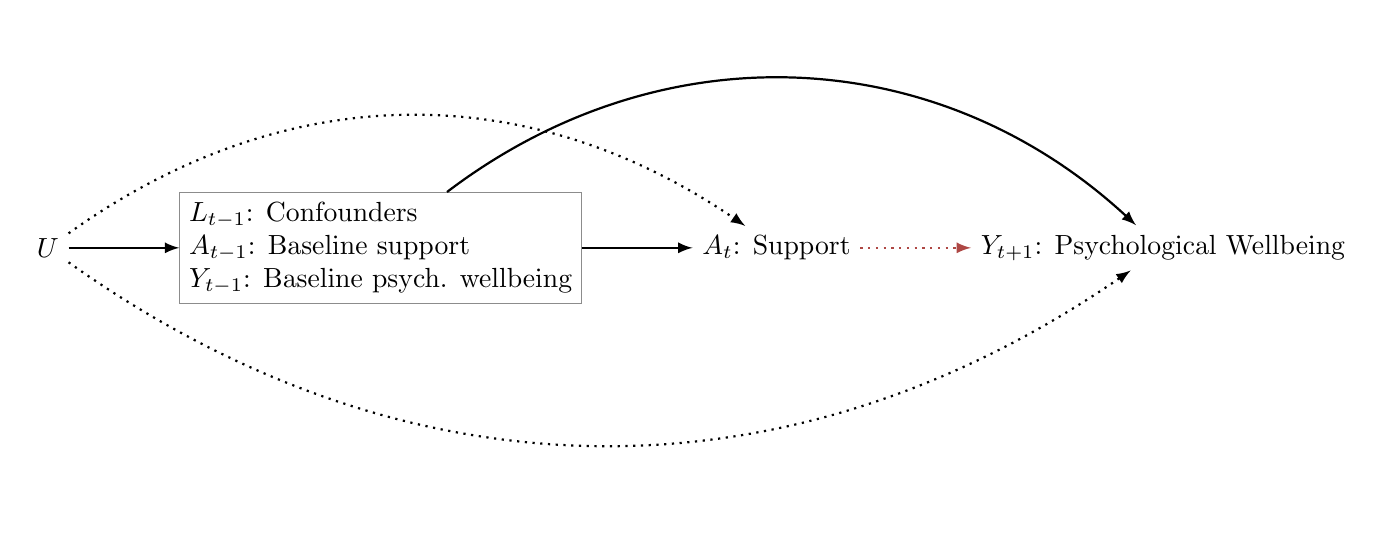
\begin{tikzpicture}[node distance=4em]
    	% Nodes
    	\node (unmeasured) {$U$};
		\node[controlled, right=of unmeasured, align=left] (confounders) {
			$L_{t - 1}$: Confounders\\
			$A_{t - 1}$: Baseline support\\
			$Y_{t - 1}$: Baseline psych. wellbeing
		};
		\node[right=of confounders] (exposure) {$A_t$: Support};
		\node[right=of exposure] (outcome) {$Y_{t+1}$: Psychological Wellbeing};
		
    	% Full arrows
		\draw[arrow] (unmeasured) to (confounders);
		\draw[arrow] (confounders) to (exposure);
		\draw[arrow, bend left=40] (confounders) to (outcome);
		
		% Dotted arrows
		\draw[dottedarrow, bend left=35] (unmeasured) to (exposure);
		\draw[dottedarrow, bend right=35] (unmeasured) to (outcome);
		\draw[dottedarrow, redtea] (exposure) to (outcome);  
    \end{tikzpicture}

\end{document}
